\documentclass[14pt]{extreport}
\input{prop/preamble.inc}


\begin{document}

\SETgroup{K3121}
\SETstudent{Сакулин Иван}
\SETteacher{Курашова С.А.}
\SETdata{05.05.2025}
\SETnumber{1.04}
\SETtitle{Исследование равноускоренного вращательного }
\SETtitleT{движения (маятник Обербека)}
\input{prop/title}

\vskip 15mm
\noindent\textbf{1. Цели работы}
\begin{enumerate}[label=\arabic*)]
    \item Проверка основного закона динамики вращения.
    \item Проверка зависимости момента инерции от положения масс относительно оси вращения.
\end{enumerate}


\noindent\textbf{2. Задачи, решаемые при выполнении работы}

\begin{enumerate}[label=\arabic*)]
    \item Измерение времени падения груза при разной массе груза и разном положении утяжелителей на крестовине.
    \item Расчёт ускорения груза, углового ускорения крестовины и момента силы натяжения нити.
    \item Расчёт момента инерции крестовины с утяжелителями и момента силы трения.
    \item Исследование зависимости момента силы натяжения нити от углового ускорения. Проверка основного закона динамики вращения.
    \item Исследование зависимости момента инерции от положения масс относительно оси вращения. Проверка теоремы Штейнера.
\end{enumerate}

\noindent\textbf{3. Объект исследования}

Равноускоренное вращательное движение.

\noindent\textbf{4. Метод экспериментального исследования}

Проведение измерений времени спуска маятника Обербека, получение экспериментальных данных, вычисление необходимых величин.

\noindent\textbf{5. Рабочие формулы и исходные данные}

\begin{itemize}
    \item Высота подъёма каретки с шайбами: $ h = ((700.0 \pm 1.0))~\text{мм} $
    \item Масса каретки: $ m_\text{каретки} = ((47.0 \pm 0.5))~\text{г} $
    \item Масса шайбы: $ m_\text{шайбы} = ((220.0 \pm 0.5))~\text{г} $
    \item Масса грузов на крестовине: $ m_\text{гр} = ((408.0 \pm 0.5))~\text{г} $
    \item Расстояние первой риски от оси: $ l_1 = ((57.0 \pm 0.5))~\text{мм} $
    \item Расстояние между рисками: $ l_0 = ((25.0 \pm 0.5))~\text{мм} $
    \item Диаметр ступицы: $ d_\text{ступицы} = ((46.0 \pm 0.5))~\text{мм} $
    \item Высота груза на крестовине: $ b = ((40.0 \pm 0.5))~\text{мм} $
\end{itemize}

Масса каретки с n шайбами:

\centerline{$m = m_\text{каретки} + n \cdot m_\text{шайбы}$}

Ускорение падения груза:

\centerline{$a = \frac{2h}{t^2}$}

Угловое ускорение крестовины:

\centerline{$\varepsilon = \frac{2a}{d_\text{ступицы}}$}

Момент силы натяжения нити:

\centerline{$M = \frac{m d_\text{ступицы}}{2}(g - a)$}

Расстояние между осью вращения и центром утяжелителя на риске n:

\centerline{$R = l_1 + (n - 1)l_0 + \frac{b}{2}$}

Зависимость $M(\varepsilon) = M_\text{тр}+I\varepsilon$.

Зависимость $I(R^2) = I_0+4m_\text{ут}R^2$.

Расчёт погрешности суммы (способ 1):

\centerline{$\Delta_z = \sqrt{ \left( \frac{\partial f}{\partial a} \Delta_a \right)^2 + \left( \frac{\partial f}{\partial b} \Delta_b \right)^2  +...}, \quad \varepsilon_z = \frac{\Delta_z}{\bar{z}} \cdot 100\%$.}

Расчёт погрешности произведения (способ 2):

\centerline{$\varepsilon_z = \sqrt{ \left( \frac{\partial \ln z}{\partial a} \Delta_a \right)^2 + \left( \frac{\partial \ln z}{\partial b} \Delta_b \right)^2 + \ldots } \cdot 100\%, \quad \Delta_z = \frac{\overline{z} \cdot \varepsilon_z}{100\%}$.}

\noindent\textbf{6. Измерительные приборы}

\begin{table}[H]
\centering
\small
\caption{Измерительные приборы}
\begin{tabular}{|l|c|c|c|}
\hline
\textbf{Наименование} & 
\textbf{Предел измерений} & 
\textbf{Цена деления} & \({\Delta_u}\) \\ \hline
Секундомер & 10 с & 0.01 с & 0.01 с \\ \hline
\end{tabular}
\end{table}

\noindent\textbf{7. Схема установки} 
% ИЛИ Перечень схем, которые составляют Приложение 1.

\begin{figure}[H]
    \centering
    \includegraphics[width=0.80\linewidth]{1.04.schemaN.png}
    \caption{Схема установки}
    \label{picture:cheme}
\end{figure}
% Состав установки:
% (1) основание,
% (2) рукоятка сцепления крестовин,
% (3) устройства принудительного трения,
% (4) поперечина,
% (5) груз крестовины,
% (6) трубчатая направляющая,
% (7) передняя крестовина,
% (8) задняя крестовина,
% (9) шайбы каретки,
% (10) каретка,
% (11) система передних стоек.

\noindent\textbf{8. Результаты прямых измерений и их обработки} 
%(таблицы, примеры расчетов).

\begin{table}[H]
\centering
\caption{Протокол измерений времени падения груза при разной массе груза и разном положении утяжелителей на крестовине}
\label{tab:direct104}
\begin{tabular}{|c|c|c|c|c|c|c|c|}
\hline
\multirow{2}{*}{\textbf{Масса}} & 
\multirow{2}{*}{\textbf{Время}} & 
\multicolumn{6}{c|}{\textbf{Положение утяжелителей}} \\ \cline{3-8}
& & 1 риска & 2 риска & 3 риска & 4 риска & 5 риска & 6 риска \\ \hline
\multirow{4}{*}{$ m_1 $}
 & $ t_1 $, с & 4.81 & 5.57 & 6.41 & 7.31 & 8.32 & 9.22 \\ \cline{2-8}
 & $ t_2 $, с & 4.94 & 5.58 & 6.46 & 7.24 & 8.30 & 9.29 \\ \cline{2-8}
 & $ t_3 $, с & 4.96 & 5.54 & 6.55 & 7.28 & 8.25 & 9.30 \\ \cline{2-8}
 & $ t_{\text{ср}} $, с & 4.90 & 5.56 & 6.47 & 7.28 & 8.29 & 9.27 \\ \hline
\multirow{4}{*}{$ m_2 $}
 & $ t_1 $, с & 3.40 & 4.01 & 4.68 & 5.28 & 6.09 & 6.76 \\ \cline{2-8}
 & $ t_2 $, с & 3.46 & 4.11 & 4.62 & 5.31 & 5.83 & 6.62 \\ \cline{2-8}
 & $ t_3 $, с & 3.53 & 3.96 & 4.76 & 5.37 & 5.89 & 6.68 \\ \cline{2-8}
 & $ t_{\text{ср}} $, с & 3.46 & 4.03 & 4.69 & 5.32 & 5.94 & 6.69 \\ \hline
\multirow{4}{*}{$ m_3 $}
 & $ t_1 $, с & 3.01 & 3.31 & 3.94 & 4.39 & 4.85 & 5.63 \\ \cline{2-8}
 & $ t_2 $, с & 2.79 & 3.31 & 3.89 & 4.40 & 4.92 & 5.51 \\ \cline{2-8}
 & $ t_3 $, с & 2.87 & 3.39 & 3.96 & 4.39 & 4.80 & 5.51 \\ \cline{2-8}
 & $ t_{\text{ср}} $, с & 2.89 & 3.34 & 3.93 & 4.393 & 4.86 & 5.55 \\ \hline
\multirow{4}{*}{$ m_4 $}
 & $ t_1 $, с & 2.40 & 2.83 & 3.37 & 3.80 & 4.13 & 4.78 \\ \cline{2-8}
 & $ t_2 $, с & 2.35 & 2.88 & 3.32 & 3.74 & 4.07 & 4.72 \\ \cline{2-8}
 & $ t_3 $, с & 2.46 & 2.89 & 3.42 & 3.73 & 4.06 & 4.78 \\ \cline{2-8}
 & $ t_{\text{ср}} $, с & 2.40 & 2.87 & 3.37 & 3.76 & 4.09 & 4.76 \\ \hline

\end{tabular}
\end{table}

\noindent\textbf{9. Расчет результатов косвенных измерений (таблицы, примеры расчетов)} 

\begin{table}[H]
\centering
\caption{Ускорение, угловое ускорение и момент силы.}
\label{tab:indirect104}
\begin{tabular}{|c|c|c|c|c|c|c|c|}
\hline
\multirow{3}{*}{\textbf{Значение}} & 
\multirow{3}{*}{$m$, г} & 
\multicolumn{6}{c|}{\textbf{Положение утяжелителей}} \\ \cline{3-8}
& & 1 риска & 2 риска & 3 риска & 4 риска & 5 риска & 6 риска \\ \hline
$a, \text{м}/\text{с}^2$ & \multirow{3}{*}{267.0} & 0.05823 & 0.04523 & 0.03341 & 0.02644 & 0.02037 & 0.01629\\ \cline{1-1} \cline{3-8}
$\varepsilon, \text{рад}/\text{с}^2$ & & 2.5317 & 1.9667 & 1.4526 & 1.1496 & 0.8857 & 0.7083\\ \cline{1-1} \cline{3-8}
$M, \text{Н}\cdot\text{м}$ & & 0.059944 & 0.060024 & 0.060096 & 0.060139 & 0.060176 & 0.060202 \\ \hline
$a, \text{м}/\text{с}^2$ & \multirow{3}{*}{487.0} & 0.11672 & 0.08634 & 0.06374 & 0.04947 & 0.03972 & 0.03131\\ \cline{1-1} \cline{3-8}
$\varepsilon, \text{рад}/\text{с}^2$ & & 5.0747 & 3.7541 & 2.7712 & 2.1507 & 1.7271 & 1.3614\\ \cline{1-1} \cline{3-8}
$M, \text{Н}\cdot\text{м}$ & & 0.108681 & 0.109021 & 0.109274 & 0.109434 & 0.109543 & 0.109637 \\ \hline
$a, \text{м}/\text{с}^2$ & \multirow{3}{*}{707.0} & 0.16762 & 0.12575 & 0.09064 & 0.07253 & 0.05935 & 0.04545\\ \cline{1-1} \cline{3-8}
$\varepsilon, \text{рад}/\text{с}^2$ & & 7.2879 & 5.4673 & 3.9411 & 3.1536 & 2.5806 & 1.9761\\ \cline{1-1} \cline{3-8}
$M, \text{Н}\cdot\text{м}$ & & 0.156949 & 0.157630 & 0.158201 & 0.158495 & 0.158710 & 0.158936 \\ \hline
$a, \text{м}/\text{с}^2$ & \multirow{3}{*}{927.0} & 0.24238 & 0.17036 & 0.12327 & 0.09920 & 0.08383 & 0.06179\\ \cline{1-1} \cline{3-8}
$\varepsilon, \text{рад}/\text{с}^2$ & & 10.5383 & 7.4071 & 5.3597 & 4.3132 & 3.6447 & 2.6865\\ \cline{1-1} \cline{3-8}
$M, \text{Н}\cdot\text{м}$ & & 0.204194 & 0.205729 & 0.206733 & 0.207246 & 0.207574 & 0.208044 \\ \hline

\end{tabular}
\end{table}

По МНК вычислим для разных положений регулировочных грузов зависимости $M(\varepsilon) = M_\text{тр}+I\varepsilon$.

\begin{itemize}
	\item Для 3 рисок: $M = 0.0182+0.017 \cdot I$.
	\item Для 3 рисок: $M = 0.0269+0.008 \cdot I$.
	\item Для 3 рисок: $M = 0.0379+0.006 \cdot I$.
	\item Для 3 рисок: $M = 0.0467+0.008 \cdot I$.
	\item Для 3 рисок: $M = 0.054+0.016 \cdot I$.
	\item Для 3 рисок: $M = 0.0752+0.008 \cdot I$.

\end{itemize}

\begin{table}[H]
\centering
\caption{Момент силы и момент инерции.}
\label{tab:indirect2104}
\begin{tabular}{|c|c|c|c|c|c|c|}
\hline
\multirow{3}{*}{\textbf{Значение}} & 
\multicolumn{6}{c|}{\textbf{Положение утяжелителей}} \\ \cline{2-7}
& 1 риска & 2 риска & 3 риска & 4 риска & 5 риска & 6 риска \\ \hline
$I, \text{кг}\cdot\text{м}^2$ & 0.0182 & 0.0269 & 0.0379 & 0.0467 & 0.054 & 0.0752 \\ \hline
$M_\text{тр}, \text{Н}\cdot\text{м}$ & 0.017 & 0.008 & 0.006 & 0.008 & 0.016 & 0.008 \\ \hline

\end{tabular}
\end{table}

Вычислим для разных положений грузов $R = l_1 + (n - 1)l_0 + \frac{b}{2}$.

\begin{table}[H]
\centering
\caption{Момент инерции и квадрат расстояния до грузов.}
\label{tab:indirect3104}
\begin{tabular}{|c|c|c|c|c|c|c|}
\hline
\multirow{3}{*}{\textbf{Значение}} & 
\multicolumn{6}{c|}{\textbf{Положение утяжелителей}} \\ \cline{2-7}
& 1 риска & 2 риска & 3 риска & 4 риска & 5 риска & 6 риска \\ \hline
$R, \text{м}$ & 0.0770 & 0.1020 & 0.1270 & 0.1520 & 0.1770 & 0.2020 \\ \hline
$R^2, \text{м}^2$ & 0.00593 & 0.01040 & 0.01613 & 0.02310 & 0.0313 & 0.0408 \\ \hline
$I, \text{кг}\cdot\text{м}^2$ & 0.0182 & 0.0269 & 0.0379 & 0.0467 & 0.054 & 0.0752 \\ \hline

\end{tabular}
\end{table}

По МНК вычислим зависимость $I(R^2) = I_0+2m_\text{ут}R^2$.

\centerline{$I = (0.011 \pm 0.005)+(1.53 \pm 0.21) \cdot R^2$}

$a = I_0 = ((0.011 \pm 0.005)) \text{кг}\cdot\text{м}^2$

$b = 4m_\text{ут} = ((1.53 \pm 0.21)) \text{кг}$, $m_\text{ут} = ((0.38 \pm 0.05)) \text{кг}$

Здесь $I_0$ - сумма моментов инерции стрежней крестовины, момента инерции ступицы и собственных центральных моментов инерции утяжелителей.

\noindent\textbf{10. Расчет погрешностей измерений (для прямых и косвенных измерений)}

Расчёт для множественного измерения с 1 риской и $m_1$.

Для времени: $\bar{t} = \frac{4.81 + 4.94 + 4.96 }{3} \approx 4.90 c$,

\centerline{$\sigma_{\bar{t}} = 0.047, \quad S(3, 0.95)=4.3, \quad \Delta_{\bar{t}} = 4.3 \cdot 0.047 = 0.2 c$,}

\centerline{$\Delta_{t} = \sqrt{(0.2)^2 + (\frac{2}{3} \cdot 0.01)^2} = 0.20 c, \quad \varepsilon_{t} = \frac{0.20}{4.90} \cdot 100\% = 4\%$}

Для массы спускающегося груза: $m = m_\text{каретки} + n \cdot m_\text{шайбы} = 267.0 \text{г}$

\centerline{$\Delta_m = \sqrt{(\Delta_{m_\text{каретки}})^2 + (n \cdot \Delta_{m_\text{шайбы}})^2} = 0.7 \text{г}, \quad \varepsilon_{m} = \frac{\Delta_m}{m} \cdot 100\% = 0.26\%$.}

Для ускорения: $a=\frac{2h}{t^2} = 0.05823 \text{м}/\text{с}^2$, 

\centerline{$\varepsilon_{a} = \sqrt{(\frac{2}{3} \cdot \frac{\Delta h}{h})^2 + (\frac{\Delta t}{t})^2} \cdot 100\% = 0.08\%, \quad \Delta_a=\frac{a \cdot \varepsilon_a}{100\%} = 5 \cdot 10^{-5} \text{м}/\text{с}^2$.}

Для углового ускорения: $\varepsilon=\frac{2a}{d_\text{ступ}} = 2.5317 \text{рад}/\text{с}^2$, 

\centerline{$\varepsilon_{\varepsilon} = \sqrt{(\frac{\Delta a}{a})^2 + (\frac{2}{3} \cdot \frac{\Delta d_\text{ступ}}{d_\text{ступ}})^2} \cdot 100\% = 0.26\%, \quad \Delta_\varepsilon=\frac{\varepsilon \cdot \varepsilon_\varepsilon}{100\%} = 0.7 \text{рад}/\text{с}^2$.}

Для момента силы натяжения нити: $M=\frac{md_\text{ступ}}{2}(g-a) = 0.059944 \text{Н}\cdot\text{м}$, 

\centerline{$\varepsilon_M = \sqrt{(\frac{\Delta m}{m})^2 + (\frac{2}{3} \cdot \frac{\Delta d_\text{ступ}}{d_\text{ступ}})^2 + (\frac{\Delta a}{g-a})^2} \cdot 100\% = 0.011\%$,}

\centerline{$\Delta_M=\frac{\varepsilon \cdot \varepsilon_\varepsilon}{100\%} = 7 \cdot 10^{-6} \text{м}/\text{с}^2$.}

Расчёт погрешности $a = I_0$ и $b = 4m_\text{ут}$ по МНК в $I(R^2) = I_0 + 4 m_\text{ут} R^2$.

\centerline{$\Delta_a=0.005 \text{кг}\cdot\text{м}^2, \varepsilon_a=50\%$; $\Delta_b=0.21 \text{кг}, \varepsilon_b=14\%$}

\noindent\textbf{11. Графики (перечень графиков)}

- Рисунок \ref{fig:g1} -- график зависимости $M(\varepsilon) = M_\text{тр}+I\varepsilon$.

- Рисунок \ref{fig:g2} -- график зависимости $I(R^2) = I_0+4m_\text{ут}R^2$.

\noindent\textbf{12. Окончательные результаты}
% \centerline{$\tau = (161\pm17)\text{c}; \quad \varepsilon = 11\%; \quad \alpha=0.95$}

Доверительные интервалы:

\centerline{$\Delta_a = 0.00005 \text{м}/\text{с}^2$}

\centerline{$\Delta_\varepsilon= 0.0021 \text{рад}/\text{с}^2$}

\centerline{$\Delta_M = 0.000007 \text{м}/\text{с}^2$}

Свободный член $I_0$ и четверть углового коэффициента $4m_\text{ут}$ зависимости $I(R^2) = I_0+4m_\text{ут}R^2$.

\centerline{$I_0 = (0.011 \pm 0.005) \text{кг} \cdot \text{м}^2, \quad \varepsilon = 50 \%, \quad \alpha = 0.95$}

\centerline{$m_\text{ут} = (0.38 \pm 0.05) \text{кг}, \quad \varepsilon = 14 \%, \quad \alpha = 0.95$}

\noindent\textbf{13. Выводы и анализ результатов работы}

В ходе выполнения лабораторной работы были исследованы зависимости момента силы натяжения нити от углового ускорения крестовины и момента инерции системы от положения грузов-утяжелителей. Уменьшение погрешностей может быть достигнуто за счёт увеличения числа измерений. Экспериментальные данные подтвердили основной закон динамики вращательного движения $M = M_\text{тр} + I \varepsilon$, так как графики $M(\varepsilon)$ для всех положений утяжелителей оказались линейными. Увеличение момента инерции $I$ с ростом расстояния $R$ до грузов согласуется с теоремой Штейнера $I = I_0 + 4 m_\text{ут} R^2$. 

\newpage
\textbf{Контрольные вопросы}

\begin{enumerate}
    \item Инерция — свойство тела сохранять состояние покоя или равномерного прямолинейного движения при отсутствии внешних сил.

    \item Угловое ускорение $\varepsilon = \frac{2a}{d}$, где $d$ -- диаметр ступицы. 

    \item Сумма моментов сил, действующих на тело $M = I \cdot \varepsilon$.

    \item Теорема Штейнера позволяет определить момент инерции тела относительно произвольной оси, если известен момент инерции относительно оси, проходящей через центр масс: $I = I_0 + m \cdot R^2$, где $I_0$ — момент инерции относительно центра масс, $R$ — расстояние между осями.

    \item Учитываются момент силы натяжения нити $M$ и момент силы трения $M_{\text{тр}}$: $I \cdot \varepsilon = M - M_{\text{тр}}$.

    \item Увеличится момент инерции системы ($I = I_0 + 4m_{\text{ут}}R^2$), что приведёт к уменьшению углового ускорения при том же моменте сил.

    \item Момент инерции — мера инертности тела при вращении. Его можно найти экспериментально: $I = \frac{M - M_{\text{тр}}}{\varepsilon}$, или теоретически через интеграл.

    \item Момент силы — векторное произведение силы на плечо. $M = [\bar{F}, \bar{r}]$ В этой работе:
    $M = \frac{m \cdot d}{2} \cdot (g - a)$,
    где $d$ — диаметр ступицы, $a$ — линейное ускорение.

    \item Момент инерции — $\text{кг} \cdot \text{м}^2$, момент силы — $\text{Н} \cdot \text{м}$.

    \item Увеличится момент инерции ($I = I_0 + 4m_{\text{ут}}R^2$), что снизит угловое ускорение. Также возрастёт коэффициент при $R^2$ в этой формуле.
\end{enumerate}

\newpage
\textbf{Приложение 1}

\begin{figure}[ht]
    \centering
    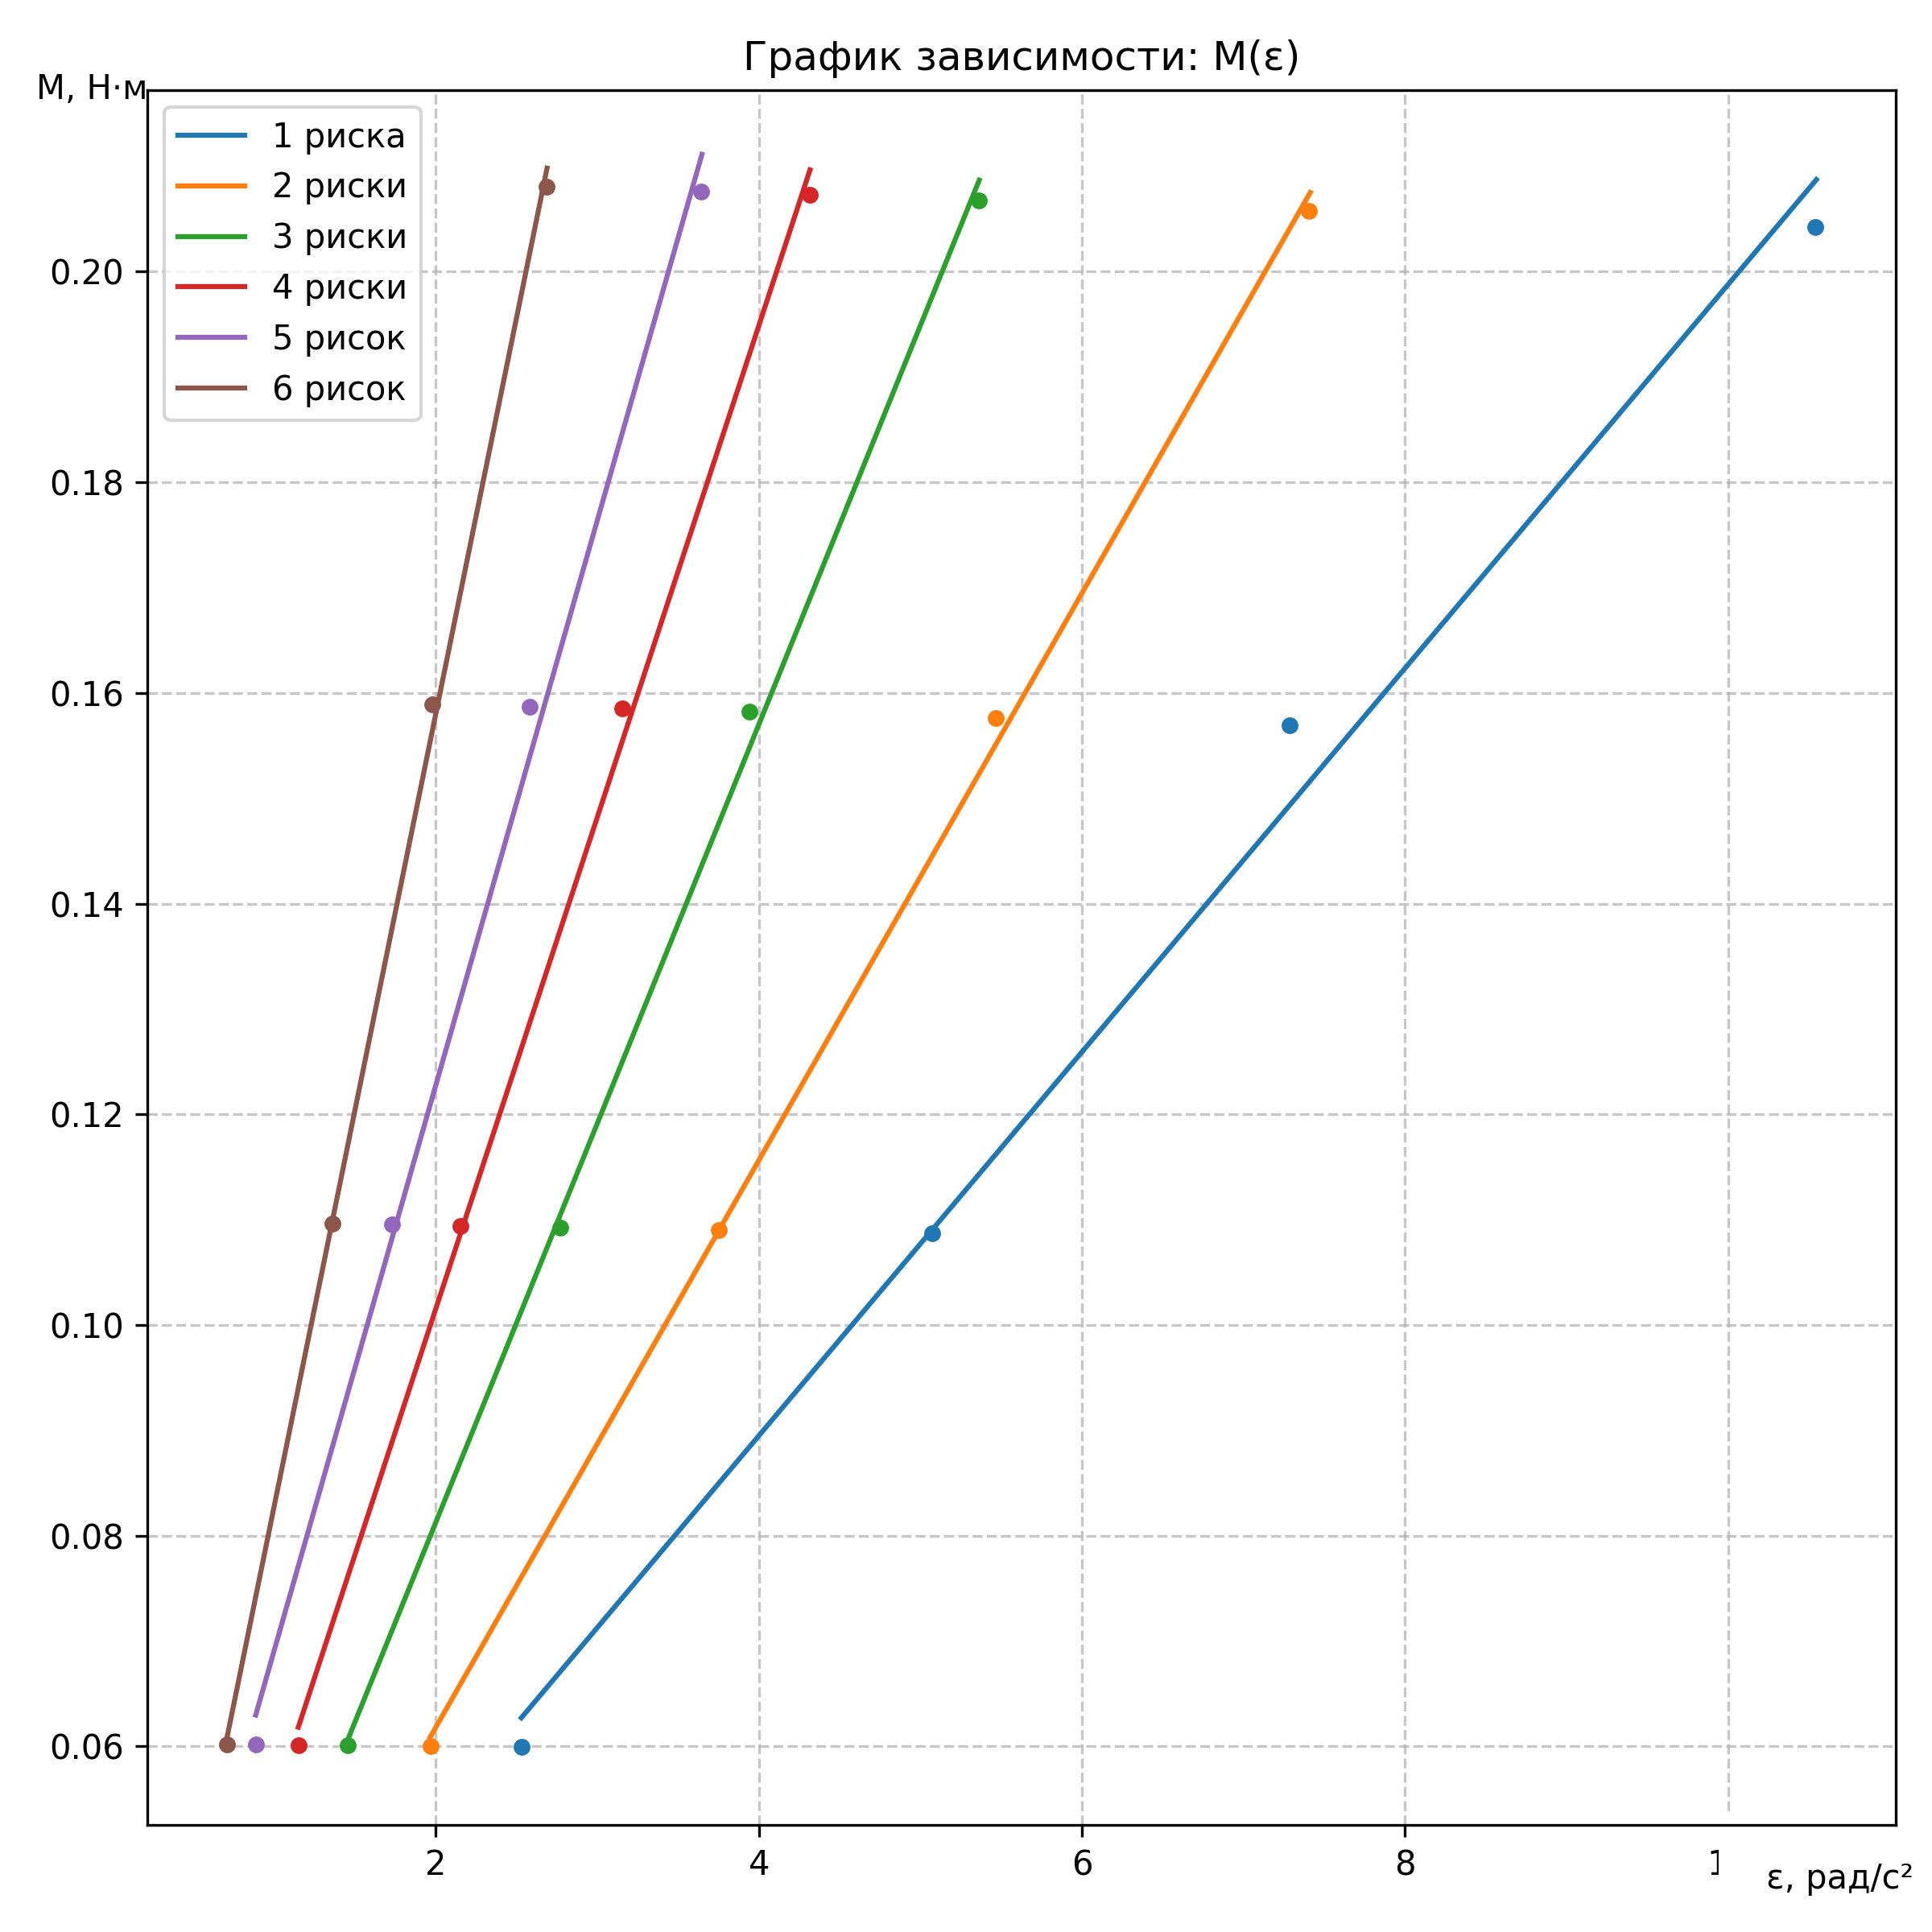
\includegraphics[width=1\linewidth]{1.04.g1.png}
    \caption{График зависимости момента силы от углового ускорения}
    \label{fig:g1}
\end{figure}

\begin{figure}
    \centering
    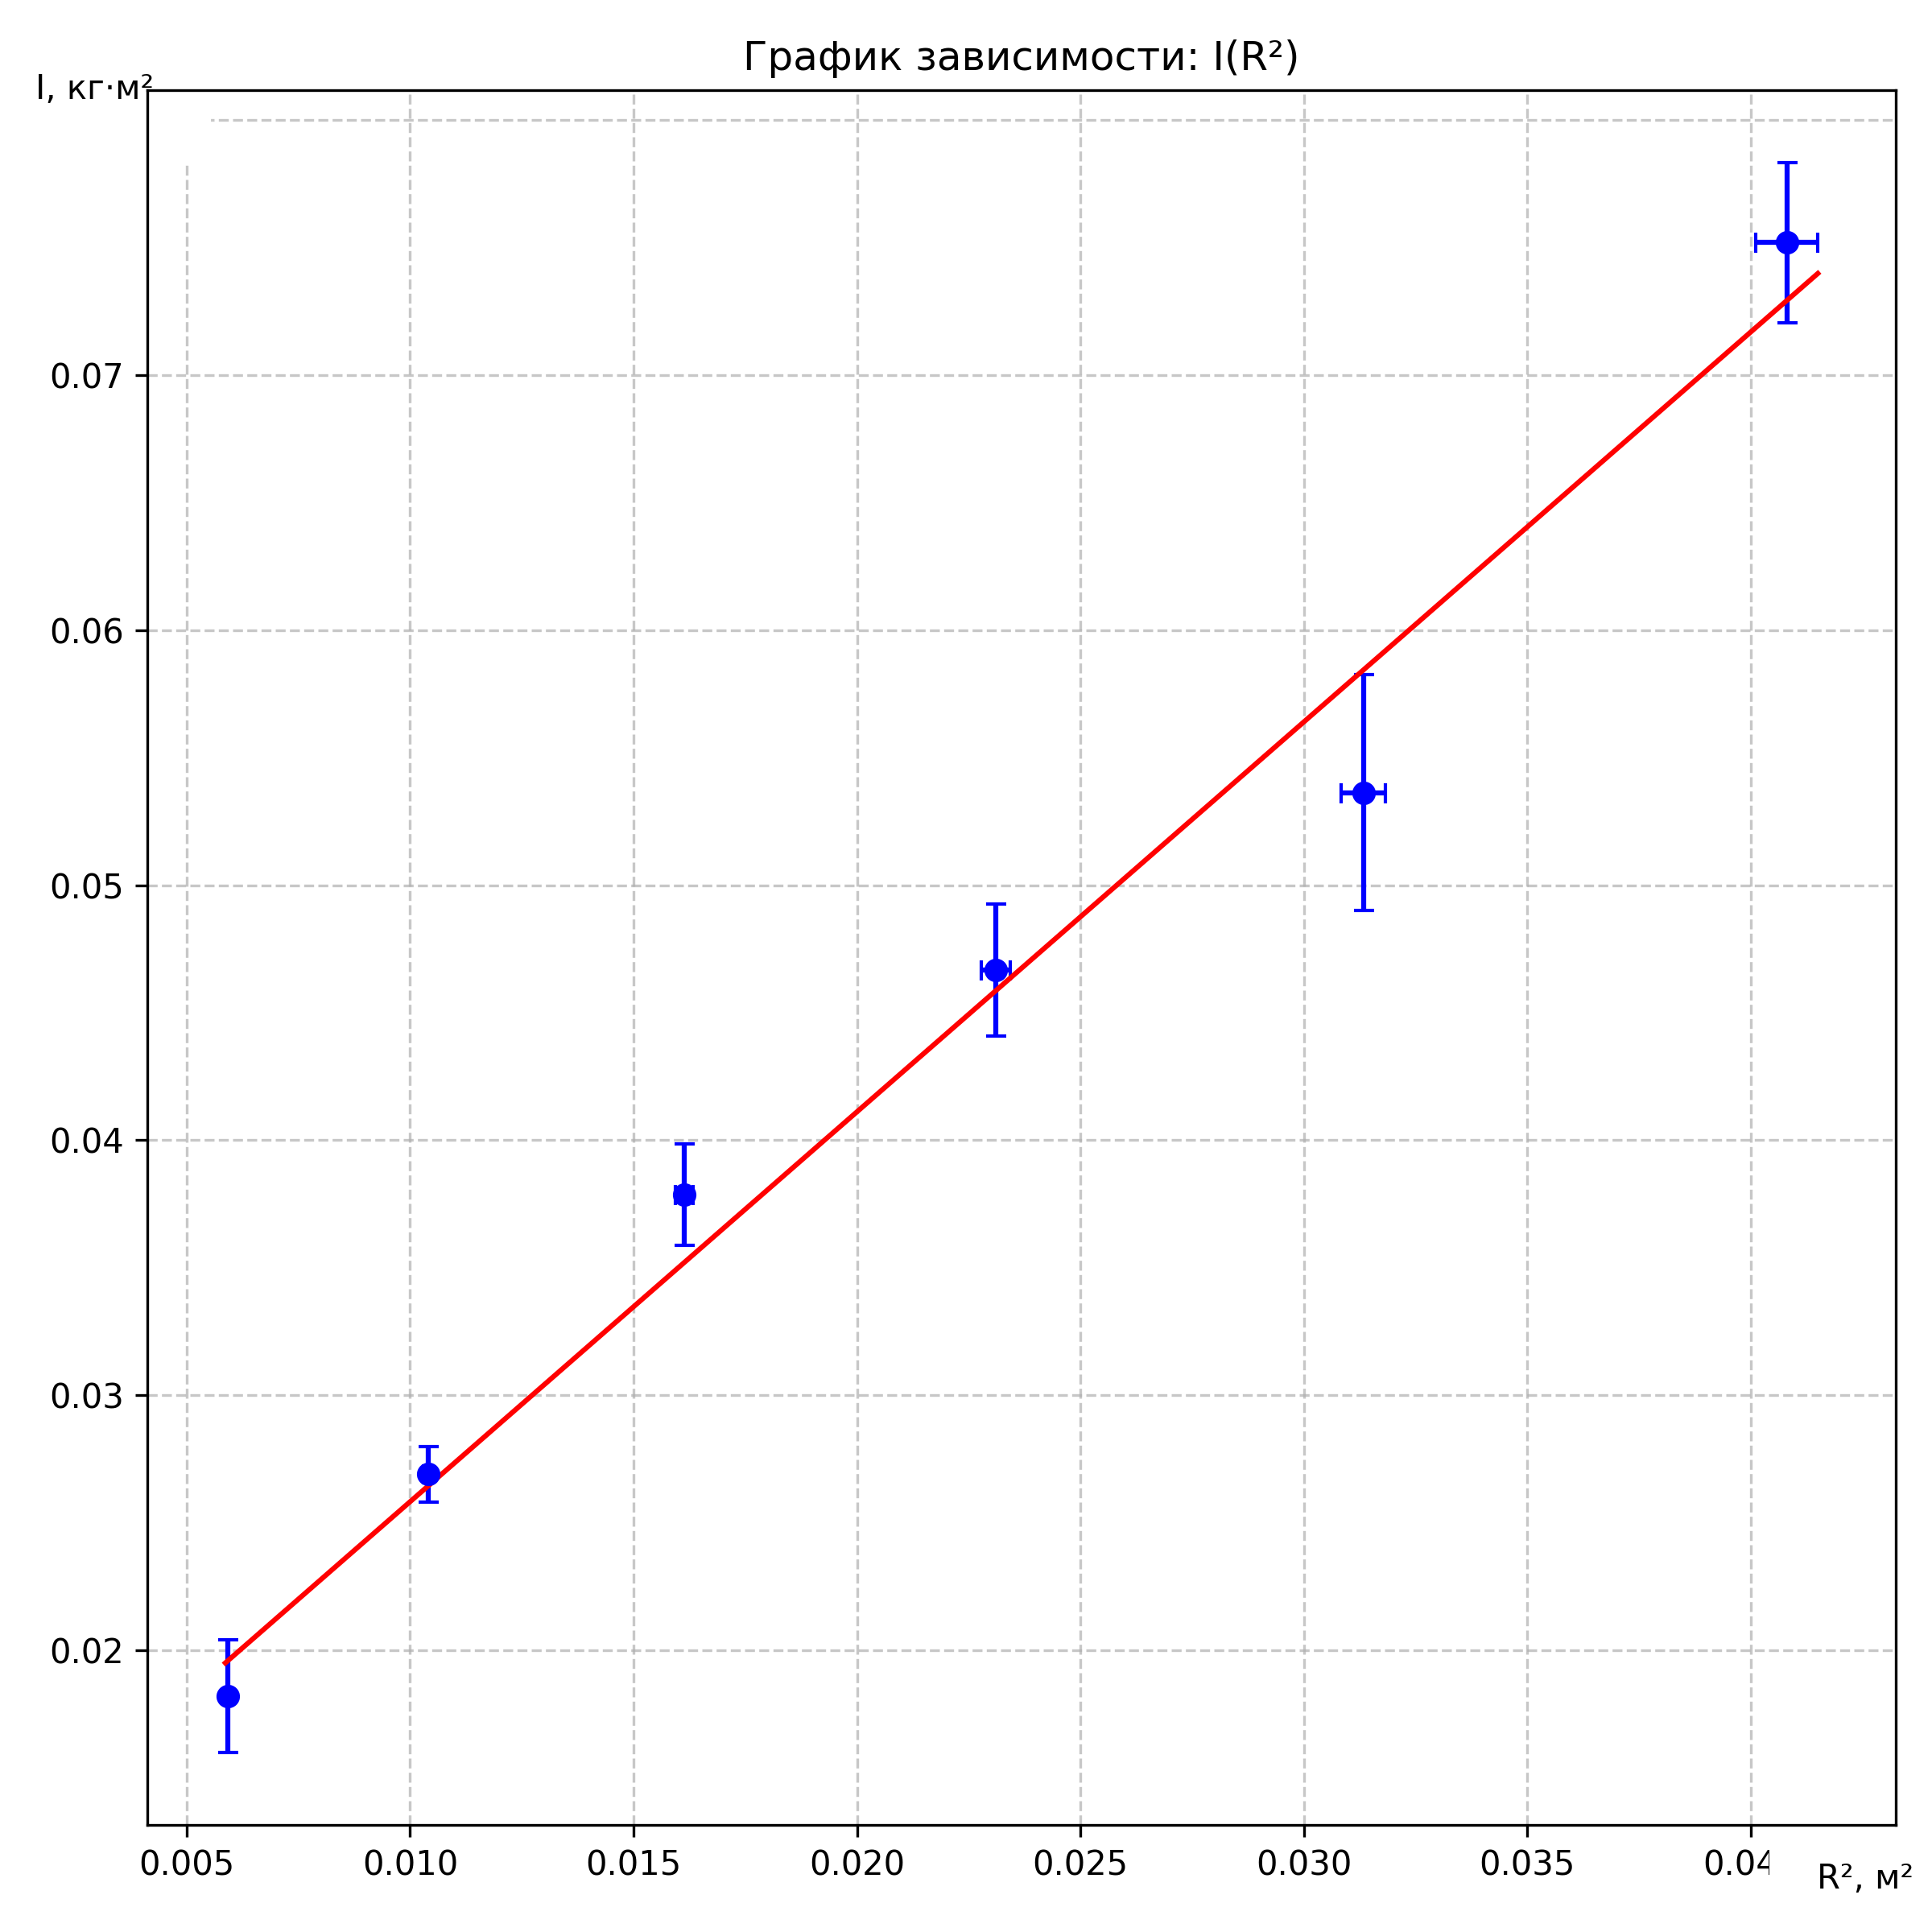
\includegraphics[width=1\linewidth]{1.04.g2.png}
    \caption{График зависимости момента инерции от квадрата расстояния до грузов.}
    \label{fig:g2}
\end{figure}

\end{document}